\documentclass[9pt,aspectratio=169]{beamer}

\usepackage[utf8]{inputenc}
\usepackage[T1]{fontenc}
\usepackage[english]{babel}
\usepackage{lmodern}
\usepackage{microtype}
\usepackage{amssymb}
\usepackage{listings}
% Shared by report.tex and presentation.tex.
\usepackage{graphicx}
\usepackage{booktabs}
\usepackage{tikz}
\usetikzlibrary{arrows.meta,positioning,fit,calc,shapes.misc}

\definecolor{todored}{HTML}{C0392B}
\definecolor{good}{HTML}{1E8449}
\definecolor{bad}{HTML}{B03A2E}
\definecolor{mesh}{HTML}{2E86C1}

% Anything the team still has to fill in. Search the .tex files for \todo.
\newcommand{\todo}[1]{{\color{todored}\textbf{[TODO:} #1\textbf{]}}}

% \placeholder{width}{height}{text}: red box where a figure will go.
\newcommand{\placeholder}[3]{%
  \fcolorbox{todored}{todored!5}{\parbox[c][#2][c]{\dimexpr#1-2\fboxsep-2\fboxrule\relax}%
    {\centering\color{todored}\small #3}}}

% \evidence{file}{width}{height}{what it should show}
% Shows evidence/<file> once it exists, a placeholder until then.
\newcommand{\evidence}[4]{%
  \IfFileExists{evidence/#1}%
    {\includegraphics[width=#2,height=#3,keepaspectratio]{evidence/#1}}%
    {\placeholder{#2}{#3}{missing \texttt{evidence/#1}\\[2pt]#4}}}

\tikzset{
  >={Stealth},
  svc/.style={draw, rounded corners, minimum width=2.3cm, minimum height=.75cm,
              font=\small\ttfamily, fill=white},
  hacked/.style={svc, draw=bad, fill=bad!12},
  proxy/.style={svc, fill=mesh!15, draw=mesh},
}

\usetikzlibrary{backgrounds}

% Warsaw with the main colour switched to #8B0002 (same as the AlgoBio deck)
\usetheme{Warsaw}
\definecolor{MainRed}{HTML}{8B0002}
\definecolor{DarkRed}{HTML}{5A0001}
\definecolor{LightRed}{HTML}{FDF2F2}
\definecolor{AccentGreen}{HTML}{1B5E20}
\definecolor{CodeBg}{HTML}{F7F7F9}

\usecolortheme[named=MainRed]{structure}
\setbeamercolor{alerted text}{fg=MainRed}
\setbeamercolor{example text}{fg=AccentGreen}
\setbeamerfont{section in head/foot}{size=\fontsize{5}{5.7}\selectfont}

% Diagram colours: green = protected by the mesh, red = attacker
\colorlet{mesh}{AccentGreen}
\colorlet{good}{AccentGreen}
\colorlet{bad}{MainRed}
\tikzset{
  svc/.style={draw=DarkRed, thick, rounded corners=3pt, fill=white,
              minimum width=2.1cm, minimum height=.65cm, font=\scriptsize\ttfamily},
  hacked/.style={svc, draw=MainRed, fill=MainRed!15, text=DarkRed},
  proxy/.style={svc, draw=AccentGreen, fill=AccentGreen!10, text=AccentGreen},
  zone/.style={draw=DarkRed!60, thick, dashed, rounded corners=4pt, fill=CodeBg},
  arr/.style={-{Stealth[scale=0.85]}, thick, draw=DarkRed},
}

\lstset{
  language=bash,
  basicstyle=\ttfamily\scriptsize,
  columns=fullflexible,
  keepspaces=true,
  keywordstyle=\color{MainRed}\bfseries,
  commentstyle=\color{gray}\itshape,
  stringstyle=\color{AccentGreen},
  backgroundcolor=\color{CodeBg},
  frame=single,
  rulecolor=\color{MainRed!30},
  showstringspaces=false,
  aboveskip=2pt, belowskip=2pt,
  xleftmargin=3pt, xrightmargin=3pt
}

% Speaker notes: uncomment ONE line below.
% \setbeameroption{show notes on second screen=right}  % slides + notes side by side (pdfpc / dual screen)
% \setbeameroption{show only notes}                    % notes only, printable

\title[Modern Service Mesh -- Stage 2]{\texorpdfstring{Modern Service Mesh -- a better way \\ to secure communication between microservices}{Modern Service Mesh -- a better way to secure communication between microservices}}
\subtitle{Stage 2: Proof of Concept}
\author[Bartoszewski, Domagała, Maziarz, Pawłoś]{\texorpdfstring{Jędrzej Bartoszewski \quad Michał Domagała \quad Kacper Maziarz \quad Mikołaj Pawłoś\\[4pt]{\small Selected Issues of Network Applications 2026/2027}}{Bartoszewski, Domagała, Maziarz, Pawłoś}}
\institute[FTIMS PŁ]{\texorpdfstring{Faculty of Technical Physics, Information Technology and Applied Mathematics\\Lodz University of Technology}{FTIMS PŁ}}
\date{November 2026}

\begin{document}

% =============================================================================
% Title (Kacper)
% =============================================================================
\begin{frame}
  \titlepage
\end{frame}
\note{Kacper. Just names and the topic, ten seconds, move on.}

% =============================================================================
\section{Problem}
% =============================================================================

\begin{frame}{Inside the cluster, everyone trusts everyone}
  \begin{columns}[T,onlytextwidth]
    \begin{column}{0.42\textwidth}
      \begin{block}{Kubernetes by default}
        \begin{itemize}\setlength{\itemsep}{3pt}
          \item Online Boutique: 11 services talking gRPC and HTTP, all \alert{plaintext}
          \item Any pod can call any other pod; nobody checks who's asking
          \item Firewalls guard the edge (North-South), and East-West traffic gets no checks at all
        \end{itemize}
      \end{block}
    \end{column}
    \begin{column}{0.55\textwidth}
      \centering
      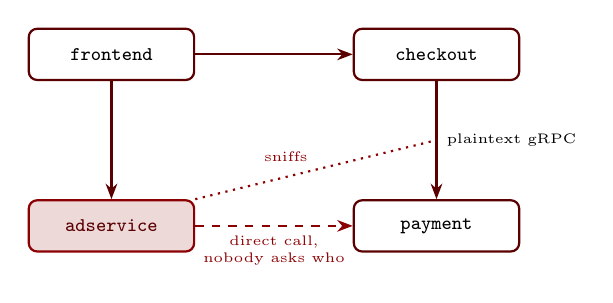
\begin{tikzpicture}[node distance=.6cm and 2.0cm]
        \node[svc]                 (fe)  {frontend};
        \node[svc, right=of fe]    (co)  {checkout};
        \node[svc, below=1.5cm of co] (pay) {payment};
        \node[hacked, below=1.5cm of fe] (ad) {adservice};
        \draw[arr] (fe) -- (co);
        \draw[arr] (co) -- node[right, font=\tiny]{plaintext gRPC} (pay);
        \draw[arr] (fe) -- (ad);
        \draw[-{Stealth[scale=0.85]}, MainRed, thick, dashed] (ad) -- node[below, font=\tiny, align=center]{direct call,\\nobody asks who} (pay);
        \draw[MainRed, thick, dotted] (ad.north east) -- node[above left=-1pt, font=\tiny]{sniffs} ($(co)!.5!(pay)$);
      \end{tikzpicture}
    \end{column}
  \end{columns}
\end{frame}
\note{Kacper. Kubernetes doesn't encrypt pod-to-pod traffic and doesn't
authenticate callers. So if someone gets into one small, boring service like
the ad service, they can read traffic passing by and send requests straight
to payments, because payments has no way of telling a legitimate checkout
call from an attacker's. That's the scenario we're building the whole project
around.}

\begin{frame}{What an attacker gets from one weak pod}
  \centering
  \vspace{4pt}
  \begin{tabular}{ll}
    \toprule
    \textbf{Attack}  & \textbf{Why it works today} \\
    \midrule
    Eavesdropping    & Traffic between pods is plaintext \\
    Impersonation    & Services have no cryptographic identity \\
    Lateral movement & Nothing restricts who may call whom \\
    \bottomrule
  \end{tabular}

  \vspace{12pt}
  \begin{alertblock}{Three gaps, three different fixes}
    Encryption, identity and access control are separate problems. Stage 2
    closes the first two; the third stays open until step 3.
  \end{alertblock}
\end{frame}
\note{Kacper. Three separate gaps, and they need separate fixes. Keep that in
mind, because our stage-2 result closes the first two and leaves the third
wide open on purpose.}

% =============================================================================
\section{Solution}
% =============================================================================

\begin{frame}{Our idea: Zero Trust, enforced by the infrastructure}
  \begin{block}{Service mesh}
    \begin{itemize}\setlength{\itemsep}{2pt}
      \item A small proxy sits next to every service (a sidecar) and handles all its traffic
      \item Proxies encrypt with mutual TLS and prove identity with certificates
      \item Policies decide which identity may call which service
      \item \textbf{No change to application code}
    \end{itemize}
  \end{block}
  \vfill
  \centering
  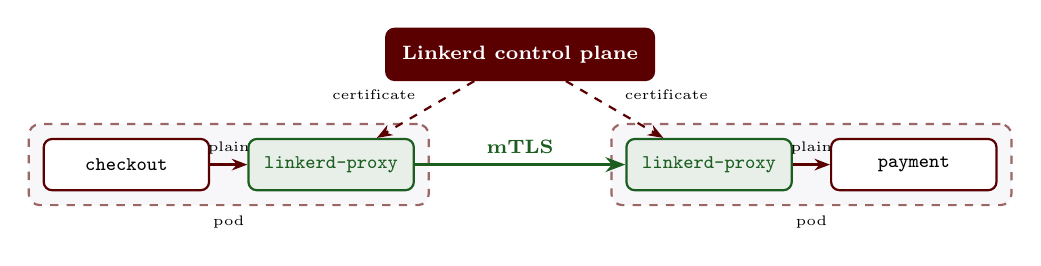
\begin{tikzpicture}[font=\scriptsize]
    \node[svc]   (a1) at (0,0)    {checkout};
    \node[proxy] (p1) at (2.6,0)  {linkerd-proxy};
    \node[proxy] (p2) at (7.4,0)  {linkerd-proxy};
    \node[svc]   (a2) at (10.0,0) {payment};
    \begin{scope}[on background layer]
      \node[zone, fit=(a1)(p1), inner sep=5pt, label={[font=\tiny]below:pod}] {};
      \node[zone, fit=(a2)(p2), inner sep=5pt, label={[font=\tiny]below:pod}] {};
    \end{scope}
    \draw[arr] (a1) -- node[above, font=\tiny]{plain} (p1);
    \draw[-{Stealth[scale=0.85]}, very thick, AccentGreen] (p1) -- node[above]{\textbf{mTLS}} (p2);
    \draw[arr] (p2) -- node[above, font=\tiny]{plain} (a2);
    \node[svc, fill=DarkRed, text=white, minimum width=3.4cm, font=\scriptsize\bfseries] (cp) at (5,1.4) {Linkerd control plane};
    \draw[arr, dashed] (cp) -- node[above left, font=\tiny]{certificate} (p1);
    \draw[arr, dashed] (cp) -- node[above right, font=\tiny]{certificate} (p2);
  \end{tikzpicture}
\end{frame}
\note{Kacper. The application keeps talking plain gRPC to localhost; the
proxy picks the traffic up and wraps it in TLS on the way out, and the
receiving proxy unwraps it. Because the mesh hands out certificates per
Kubernetes ServiceAccount, each service gets its own identity, and that
identity is what the policies in step 3 will refer to.}

\begin{frame}{Why not the alternatives?}
  \centering
  \vspace{4pt}
  \begin{tabular}{lp{8.5cm}}
    \toprule
    \textbf{Option}            & \textbf{Problem for us} \\
    \midrule
    TLS inside each app        & Code changes in 5 languages, certificates managed by hand \\
    Kubernetes NetworkPolicies & IP/port rules only: no encryption, no identity \\
    Istio                      & Does everything, but heavier to run and to learn on a laptop cluster \\
    \midrule
    \textbf{Linkerd}           & \textcolor{AccentGreen}{Automatic mTLS, Rust micro-proxy, small enough for k3d} \\
    \bottomrule
  \end{tabular}
\end{frame}
\note{Kacper. Online Boutique is written in Go, C\#, Node.js, Python and Java,
so doing TLS in the apps means five implementations. NetworkPolicies are good
at ``this pod may reach that port'', but they work on IPs, so they don't
encrypt anything and can't tell who is really on the other end. Istio could
do this job too; we went with Linkerd because it's lighter and simpler, which
matters when four of us run it on our own machines.}

\begin{frame}{The stack}
  \begin{columns}[T,onlytextwidth]
    \begin{column}{0.40\textwidth}
      \begin{block}{Tools}
        \begin{itemize}\setlength{\itemsep}{3pt}
          \item \textbf{k3d:} Kubernetes in Docker containers, free and local
          \item \textbf{Online Boutique v0.10.7:} a realistic shop we attack instead of writing our own
          \item \textbf{Linkerd:} mTLS, identity, authorization policies
          \item \textbf{Prometheus + Grafana:} proxy metrics, dashboards for allowed vs.\ denied traffic
        \end{itemize}
      \end{block}
    \end{column}
    \begin{column}{0.57\textwidth}
      \centering
      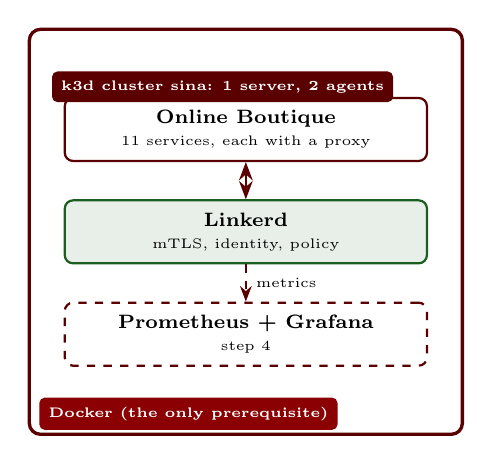
\begin{tikzpicture}[font=\scriptsize,
          box/.style={svc, font=\scriptsize, align=center, minimum width=4.6cm, minimum height=.8cm}]
        \node[box]                                      (ob)  at (0,0)    {\textbf{Online Boutique}\\\tiny 11 services, each with a proxy};
        \node[box, draw=AccentGreen, fill=AccentGreen!10] (l5d) at (0,-1.3) {\textbf{Linkerd}\\\tiny mTLS, identity, policy};
        \node[box, dashed]                              (mon) at (0,-2.6) {\textbf{Prometheus + Grafana}\\\tiny step 4};
        \draw[arr, <->] (ob) -- (l5d);
        \draw[arr, dashed] (l5d) -- node[right, font=\tiny]{metrics} (mon);
        \begin{scope}[on background layer]
          \node[zone, fit=(ob)(l5d)(mon), inner sep=8pt, inner ysep=12pt] (k3d) {};
          \node[draw=DarkRed, very thick, rounded corners=4pt, fill=white, fit=(k3d), inner sep=4pt, inner ysep=12pt] (dock) {};
        \end{scope}
        \node[fill=DarkRed, text=white, font=\tiny\bfseries, rounded corners=2pt, anchor=north west]
          at ([xshift=4pt,yshift=-3pt]k3d.north west) {k3d cluster sina: 1 server, 2 agents};
        \node[fill=MainRed, text=white, font=\tiny\bfseries, rounded corners=2pt, anchor=south west]
          at ([xshift=4pt,yshift=2pt]dock.south west) {Docker (the only prerequisite)};
      \end{tikzpicture}
    \end{column}
  \end{columns}
\end{frame}
\note{Mikołaj. Walk the diagram from the outside in. Only Docker is a
prerequisite; everything else is pulled in by our scripts. Prometheus and
Grafana come in at step 4, mention that they're planned, not done.}

% =============================================================================
\section{Progress}
% =============================================================================

\begin{frame}{Where we are}
  \centering
  \vspace{4pt}
  \begin{tabular}{lll}
    \toprule
    \textbf{Step} & \textbf{When} & \textbf{Status} \\
    \midrule
    1. k3d cluster + Online Boutique      & weeks 3--4         & \textcolor{AccentGreen}{\textbf{done}} \\
    2. Linkerd + mTLS proof of concept    & weeks 5--6 (6.11)  & \textcolor{AccentGreen}{\textbf{done}} \\
    3. Zero-Trust authorization policies  & week 7             & \alert{next} \\
    4. Prometheus + Grafana               & week 8             & planned \\
    5. Attack simulation                  & week 9 (27.11)     & planned \\
    \bottomrule
  \end{tabular}
\end{frame}
\note{Mikołaj. We're on schedule: both PoC steps are done by the 6.11
deadline.}

\begin{frame}[fragile]{Step 1: one command, any laptop}
  \begin{columns}[T,onlytextwidth]
    \begin{column}{0.44\textwidth}
      \begin{block}{Setup}
\begin{lstlisting}
./setup.sh                    # Linux / macOS
powershell -File .\setup.ps1  # Windows
\end{lstlisting}
        \begin{itemize}\setlength{\itemsep}{2pt}
          \item Only Docker needed; k3d v5.9.0, kubectl v1.37.2 and Linkerd edge-26.11.1 land in \texttt{./.tools/}
          \item Safe to re-run; shop at \texttt{localhost:8080}
        \end{itemize}
      \end{block}
    \end{column}
    \begin{column}{0.54\textwidth}
\begin{lstlisting}[language={}, morecomment={[l]{\#}}, basicstyle=\ttfamily\fontsize{6}{7.2}\selectfont]
$ ./setup.sh
INFO[0027] Cluster 'sina' created successfully!
deployment.apps/adservice created
service/adservice created
serviceaccount/adservice created
deployment.apps/shippingservice created
# ... same for the other 10 services
\end{lstlisting}
    \end{column}
  \end{columns}
  \vspace{4pt}
\begin{lstlisting}[language={}, morecomment={[l]{\#}}, basicstyle=\ttfamily\fontsize{6}{7.2}\selectfont]
NAME                                     READY   STATUS    RESTARTS   AGE
adservice-854578d668-xv5ls               1/1     Running   0          47s
checkoutservice-7c546c97fb-g4d2z         1/1     Running   0          47s
frontend-96b686b67-psvgp                 1/1     Running   0          47s
paymentservice-9698c4f8d-fccxd           1/1     Running   0          46s
# ... 12 pods in total, all 1/1 Running: one container each, no proxy yet
\end{lstlisting}
\end{frame}
\note{Mikołaj. This is a fresh run on my machine from before we added the
mesh: the cluster was up after 27 seconds, and all 12 pods were Running less
than a minute after that. We
pinned every version so all four of us run exactly the same thing, no matter
what's installed locally, and it needs no admin rights. Point at the READY
column: every pod is 1/1, one container. Now that step 2 is in the script, the
same command ends with 2/2, because each pod gets its Linkerd proxy. The README
also covers the failures we expect: pods stuck Pending when Docker has too little memory,
WSL2 on Windows, and Podman instead of Docker on Linux.}

\begin{frame}{Step 1: the shop, running locally}
  \centering
  \evidence{00-shop.png}{\textwidth}{6.2cm}{Online Boutique at \texttt{localhost:8080}}

  \vspace{4pt}
  {\small Online Boutique on our k3d cluster: 12 pods. Without the mesh, every call between them is plaintext}
\end{frame}
\note{Mikołaj. This is what the script ends with: the shop at localhost:8080,
served by the frontend through the k3d load balancer. In step 1, with no mesh,
every request it makes behind the scenes, from the cart to checkout to payment,
crossed the cluster in plaintext. That's the starting point for Jędrzej's
part.}

\begin{frame}{Step 2: is the traffic encrypted?}
  \begin{columns}[T,onlytextwidth]
    \begin{column}{0.49\textwidth}
      \centering
      \textbf{\texttt{linkerd viz edges}}\\[4pt]
      \evidence{04-edges.png}{\linewidth}{5cm}{every row SECURED}
    \end{column}
    \begin{column}{0.49\textwidth}
      \centering
      \textbf{\texttt{linkerd viz tap}}\\[4pt]
      \evidence{05-tap.png}{\linewidth}{5cm}{checkout $\to$ payment, \texttt{tls=true}}
    \end{column}
  \end{columns}
\end{frame}
\note{Jędrzej. Linkerd edge-26.11.1, installed with the CLI by our setup
scripts, which also deploy the shop through linkerd inject, so every pod starts
with its proxy. Edges shows all 16 service-to-service connections as secured;
tap shows individual live requests from checkout to payment, each one marked
tls=true.}

\begin{frame}{Same request, before and after}
  \begin{columns}[T,onlytextwidth]
    \begin{column}{0.49\textwidth}
      \centering
      \textcolor{MainRed}{\textbf{Without mesh}}\\[4pt]
      \evidence{06-before.png}{\linewidth}{5cm}{tcpdump, readable payload}
    \end{column}
    \begin{column}{0.49\textwidth}
      \centering
      \textcolor{AccentGreen}{\textbf{With mesh}}\\[4pt]
      \evidence{07-after.png}{\linewidth}{5cm}{tcpdump, TLS noise}
    \end{column}
  \end{columns}
\end{frame}
\note{Jędrzej. We took paymentservice out of the mesh and captured its
traffic from the node. Without the proxy you can read the request contents
straight off the wire: the test card number and the currency, in all five test
orders. Put it back in the mesh, run the same capture with five more orders, and
neither string shows up anywhere: it's unreadable traffic between the proxies
on port 4143. No code changed between the
two screenshots, only one annotation.}

\begin{frame}{What surprised us}
  \begin{alertblock}{Encrypted $\neq$ protected}
    Any pod can still call \texttt{paymentservice}: Linkerd's default inbound
    policy is \texttt{all-unauthenticated}, so even unmeshed, plaintext
    clients get in.
  \end{alertblock}
  \begin{block}{Smaller lessons}
    \begin{itemize}\setlength{\itemsep}{2pt}
      \item Traefik, on by default in k3s, clashes with the Gateway API CRDs Linkerd needs, so we disabled it
      \item Showing encryption took more work than turning it on: distroless images,
        \texttt{runAsNonRoot}, so we captured from the node
      \item A full system drive hung Docker Desktop, and the setup script with it
    \end{itemize}
  \end{block}
\end{frame}
\note{Jędrzej. The first point is the big one. After step 2 an attacker can't
read the traffic anymore, but they can still send requests to payments,
because the default inbound policy is all-unauthenticated. We tested it with
a pod outside the mesh and a pod using the adservice identity, and both reached
payment and cart. So we fixed eavesdropping and impersonation, and lateral
movement is still open. On proving it: the app images have no shell, and they
refuse root containers,
so we had to capture from the node. Capture inside the pod and you'd see
plaintext anyway on loopback, between the app and its own proxy.}

% =============================================================================
\section{Next steps}
% =============================================================================

\begin{frame}{Next: close the door (steps 3 and 5)}
  \begin{columns}[c,onlytextwidth]
    \begin{column}{0.45\textwidth}
      \begin{block}{Authorization policies}
        \begin{itemize}\setlength{\itemsep}{2pt}
          \item Default-deny for the namespace, then allow only the calls the app really makes
          \item Only the \texttt{checkoutservice} identity may call \texttt{paymentservice}
        \end{itemize}
      \end{block}
      \begin{exampleblock}{Attack simulation}
        Same attack twice, from an outside pod and from a hijacked
        \texttt{adservice}: it goes through now, and should get
        \texttt{PermissionDenied} after.
      \end{exampleblock}
    \end{column}
    \begin{column}{0.52\textwidth}
      \centering
      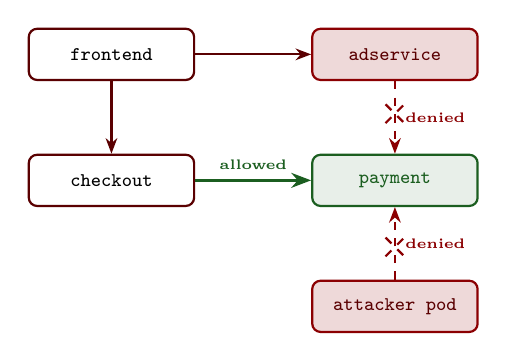
\begin{tikzpicture}[font=\scriptsize]
        \node[svc]    (fe)  at (0,0)      {frontend};
        \node[svc]    (co)  at (0,-1.6)   {checkout};
        \node[proxy]  (pay) at (3.6,-1.6) {payment};
        \node[hacked] (ad)  at (3.6,0)    {adservice};
        \node[hacked] (atk) at (3.6,-3.2) {attacker pod};
        \draw[arr] (fe) -- (co);
        \draw[arr] (fe) -- (ad);
        \draw[-{Stealth[scale=0.85]}, AccentGreen, very thick] (co) -- node[above, font=\tiny\bfseries]{allowed} (pay);
        \draw[-{Stealth[scale=0.85]}, MainRed, thick, dashed] (ad) -- node[pos=.45, cross out, draw=MainRed, thick,
              minimum size=6pt, inner sep=0pt]{} node[right, pos=.5, font=\tiny\bfseries]{denied} (pay);
        \draw[-{Stealth[scale=0.85]}, MainRed, thick, dashed] (atk) -- node[pos=.45, cross out, draw=MainRed, thick,
              minimum size=6pt, inner sep=0pt]{} node[right, pos=.5, font=\tiny\bfseries]{denied} (pay);
      \end{tikzpicture}

      {\tiny The other 12 allowed edges of the call graph are left out.}
    \end{column}
  \end{columns}
\end{frame}
\note{Michał. Each Online Boutique service already runs under its own
ServiceAccount, so each one gets its own mesh identity, and that's what we
write the policies against. Two things we have to keep working: the frontend
accepts traffic from outside the mesh, and the loadgenerator has to keep
reaching it.}

\begin{frame}{Next: make it visible (step 4)}
  \begin{block}{Observability}
    \begin{itemize}\setlength{\itemsep}{3pt}
      \item Prometheus scrapes every proxy: request counts, latency, TLS status, denials
      \item Grafana dashboard showing allowed vs.\ denied requests per service
      \item The attack from step 5 should show up on it live
    \end{itemize}
  \end{block}
  \begin{block}{Plan}
    Start with the Prometheus bundled with \texttt{linkerd-viz} and add Grafana;
    move to a separate Prometheus if it limits us
  \end{block}
\end{frame}
\note{Kacper. linkerd-viz ships its own Prometheus, but it's meant for demos
and keeps only a few hours of data, and Grafana stopped being bundled with
Linkerd a while ago. We'll start with that bundled Prometheus and add Grafana,
and move to a separate Prometheus if it limits us. So step 4 is mostly about
building one dashboard that makes the attack obvious.}

% =============================================================================
% Closing
% =============================================================================
\begin{frame}
  \centering
  \vspace{1.2cm}
  \begin{beamercolorbox}[sep=14pt,center,shadow=true,rounded=true]{title}
    {\LARGE \textbf{Thank you}}\\[8pt]
    {\large Questions?}
  \end{beamercolorbox}
  \vspace{12pt}

  {\small Repo: \texttt{github.com/Mxkyp/selected-network-issues}}
\end{frame}
\note{Everyone. Backup: have the cluster running on one laptop in case
someone asks to see tap live.}

\end{document}
